\documentclass[portrait,final,paperwidth=31truein,paperheight=38truein,fontscale=0.35, margin=1truein]{baposter}

\usepackage{calc}
\usepackage{graphicx}
\usepackage{amsmath}
\usepackage{amssymb}
\usepackage{relsize}
\usepackage{multirow}
\usepackage{rotating}
\usepackage{bm}
\usepackage{bbm}
\usepackage{url}

\usepackage{graphicx}
\usepackage{multicol}

%\usepackage{times}
%\usepackage{helvet}
%\usepackage{bookman}
\usepackage{palatino}

\newcommand{\captionfont}{\footnotesize}

\graphicspath{{images/}{../images/}}
\usetikzlibrary{calc}

\newcommand{\SET}[1]  {\ensuremath{\mathcal{#1}}}
\newcommand{\MAT}[1]  {\ensuremath{\boldsymbol{#1}}}
\newcommand{\VEC}[1]  {\ensuremath{\boldsymbol{#1}}}
\newcommand{\Video}{\SET{V}}
\newcommand{\video}{\VEC{f}}
\newcommand{\track}{x}
\newcommand{\Track}{\SET T}
\newcommand{\LMs}{\SET L}
\newcommand{\lm}{l}
\newcommand{\PosE}{\SET P}
\newcommand{\posE}{\VEC p}
\newcommand{\negE}{\VEC n}
\newcommand{\NegE}{\SET N}
\newcommand{\Occluded}{\SET O}
\newcommand{\occluded}{o}

%%%%%%%%%%%%%%%%%%%%%%%%%%%%%%%%%%%%%%%%%%%%%%%%%%%%%%%%%%%%%%%%%%%%%%%%%%%%%%%%
%%%% Some math symbols used in the text
%%%%%%%%%%%%%%%%%%%%%%%%%%%%%%%%%%%%%%%%%%%%%%%%%%%%%%%%%%%%%%%%%%%%%%%%%%%%%%%%

%%%%%%%%%%%%%%%%%%%%%%%%%%%%%%%%%%%%%%%%%%%%%%%%%%%%%%%%%%%%%%%%%%%%%%%%%%%%%%%%
% Multicol Settings
%%%%%%%%%%%%%%%%%%%%%%%%%%%%%%%%%%%%%%%%%%%%%%%%%%%%%%%%%%%%%%%%%%%%%%%%%%%%%%%%
\setlength{\columnsep}{1.5em}
\setlength{\columnseprule}{0mm}

%%%%%%%%%%%%%%%%%%%%%%%%%%%%%%%%%%%%%%%%%%%%%%%%%%%%%%%%%%%%%%%%%%%%%%%%%%%%%%%%
% Save space in lists. Use this after the opening of the list
%%%%%%%%%%%%%%%%%%%%%%%%%%%%%%%%%%%%%%%%%%%%%%%%%%%%%%%%%%%%%%%%%%%%%%%%%%%%%%%%
\newcommand{\compresslist}{%
\setlength{\itemsep}{1pt}%
\setlength{\parskip}{0pt}%
\setlength{\parsep}{0pt}%
}

%%%%%%%%%%%%%%%%%%%%%%%%%%%%%%%%%%%%%%%%%%%%%%%%%%%%%%%%%%%%%%%%%%%%%%%%%%%%%%
%%% Begin of Document
%%%%%%%%%%%%%%%%%%%%%%%%%%%%%%%%%%%%%%%%%%%%%%%%%%%%%%%%%%%%%%%%%%%%%%%%%%%%%%

\begin{document}

%%%%%%%%%%%%%%%%%%%%%%%%%%%%%%%%%%%%%%%%%%%%%%%%%%%%%%%%%%%%%%%%%%%%%%%%%%%%%%
%%% Here starts the poster
%%%---------------------------------------------------------------------------
%%% Format it to your taste with the options
%%%%%%%%%%%%%%%%%%%%%%%%%%%%%%%%%%%%%%%%%%%%%%%%%%%%%%%%%%%%%%%%%%%%%%%%%%%%%%
% Define some colors

%\definecolor{lightblue}{cmyk}{0.83,0.24,0,0.12}
\definecolor{lightblue}{rgb}{0.145,0.6666,1}


\hyphenation{resolution occlusions}
%%
\begin{poster}%
  % Poster Options
  {
  % Show grid to help with alignment
  grid=false,
  columns = 2,
  % Column spacing
  colspacing=1em,
  % Color style
  bgColorOne=white,
  bgColorTwo=white,
  borderColor=lightblue,
  headerColorOne=black,
  headerColorTwo=lightblue,
  headerFontColor=white,
  boxColorOne=white,
  boxColorTwo=lightblue,
  % Format of textbox
  textborder=roundedleft,
  % Format of text header
  eyecatcher=true,
  headerborder=closed,
  headerheight=0.1\textheight,
%  textfont=\sc, An example of changing the text font
  headershape=roundedright,
  headershade=shadelr,
  headerfont=\Large\bf\textsc, %Sans Serif
  textfont={\setlength{\parindent}{1.5em}},
  boxshade=plain,
%  background=shade-tb,
  background=plain,
  linewidth=2pt
  }
  % Eye Catcher
  {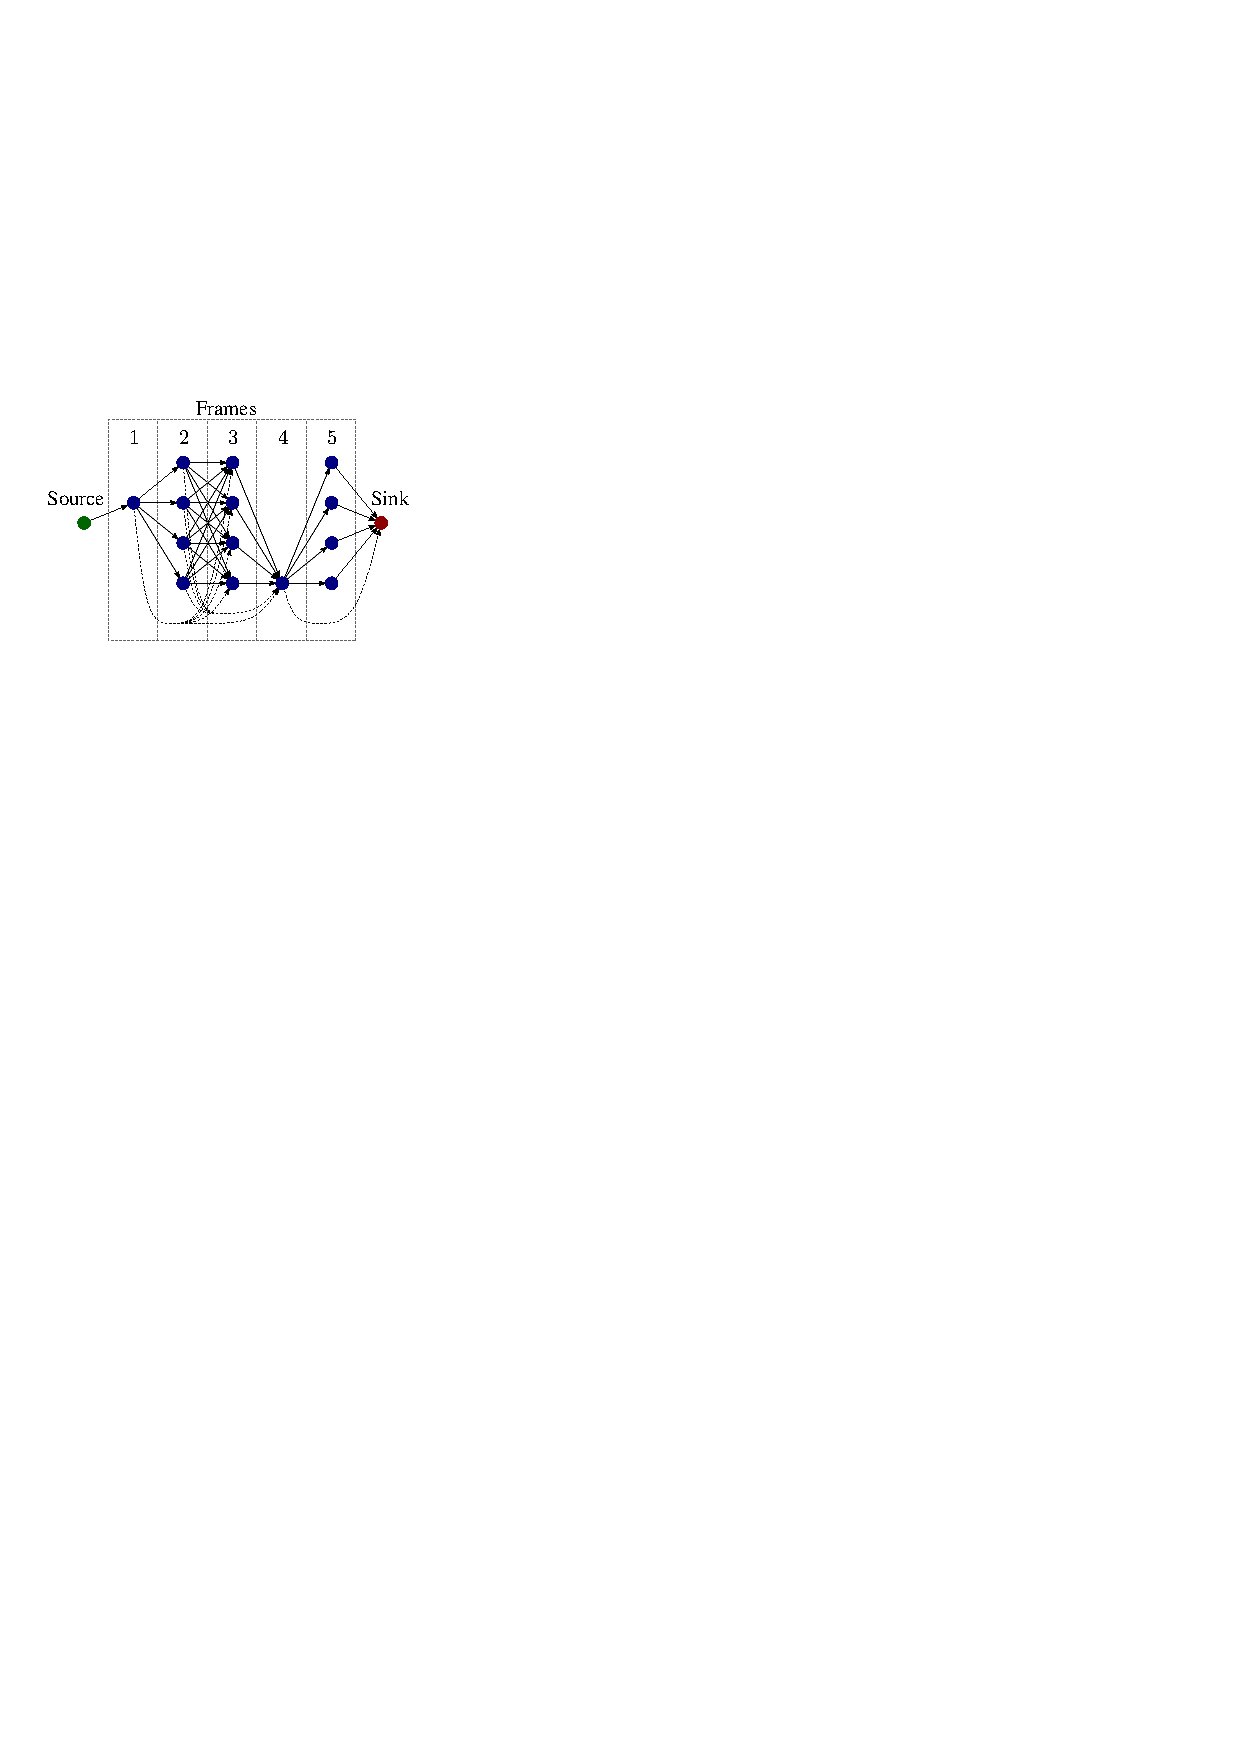
\includegraphics[height=5.5em]{images/graph_occluded.pdf}}
  % Title
  {\bf\textsc{Identification of Songbird Species \\ in Field Recordings}\vspace{0.5em}}
  % Authors
  {\textsc{Hsiao-Yu Tung, De-An Huang, Xiao-Feng Xie, Yurui Zhou, Joseph Russino }}
  % {\textsc{
  %   Hsiao-Yu Tung \\
  %   %Carnegie Mellon University\\
  %   %\texttt{htung@andrew} \\
  %   \texttt{htung@andrew.cmu.edu} \\
  %   htung \\
  %   \And
  %   De-An Huang \\
  %   %Carnegie Mellon University\\
  %   %\texttt{deanh@andrew} \\
  %   \texttt{deanh@andrew.cmu.edu} \\
  %   deanh \\
  %   \And
  %   Xiao-Feng Xie \\
  %   %Carnegie Mellon University\\
  %   %\texttt{xfxie@cs} \\
  %   \texttt{xfxie@cs.cmu.edu} \\
  %   xfxie \\
  %   \And
  %   Yurui Zhou\\
  %   %\texttt{yuruiz@andrew}\\
  %   \texttt{yuruiz@andrew.cmu.edu}\\
  %   yuruiz \\
  %   \And
  %   Joseph Russino\\
  %   %\texttt{yuruiz@andrew}\\
  %   \texttt{jrussino@rec.ri.cmu.edu}\\
  %   jrussino \\
  %   }}
  % University logo
  {% The makebox allows the title to flow into the logo, this is a hack because of the L shaped logo.
    
\includegraphics[height=8.0em]{images/logo}
  }


%%%%%%%%%%%%%%%%%%%%%%%%%%%%%%%%%%%%%%%%%%%%%%%%%%%%%%%%%%%%%%%%%%%%%%%%%%%%%%
%%% Now define the boxes that make up the poster
%%%---------------------------------------------------------------------------
%%% Each box has a name and can be placed absolutely or relatively.
%%% The only inconvenience is that you can only specify a relative position
%%% towards an already declared box. So if you have a box attached to the
%%% bottom, one to the top and a third one which should be in between, you
%%% have to specify the top and bottom boxes before you specify the middle
%%% box.
%%%%%%%%%%%%%%%%%%%%%%%%%%%%%%%%%%%%%%%%%%%%%%%%%%%%%%%%%%%%%%%%%%%%%%%%%%%%%%

%%%%%%%%%%%%%%%%%%%%%%%%%%%%%%%%%%%%%%%%%%%%%%%%%%%%%%%%%%%%%%%%%%%%%%%%%%%%%%
\headerbox{Introduction}{name=Introduction,column=0,row=0}{
%%%%%%%%%%%%%%%%%%%%%%%%%%%%%%%%%%%%%%%%%%%%%%%%%%%%%%%%%%%%%%%%%%%%%%%%%%%%%%
It is important to gain a better understanding about the climate and ecological changes in the world. One way to address this is to study seasonal migration patterns in songbird populations, since birds respond quickly to environmental changes
During migratory periods, many species of songbirds use flight calls, which are species-specific and are distinct from other vocalizations. Therefore, flight calls information can be used to determine the relative abundance of species and is important to understand long-term population trends. Due to costly human effort to collect data about birds in traditional methods, using machine learing (ML) methods to identify bird species from continuous audio recordings has been a hot topic in in recent conference competitions. Although there are some recent advances  it is still an open ML problem to reliably identify bird sounds in field recordings data due to simultaneously vocalizing birds and various background noise.

}

%%%%%%%%%%%%%%%%%%%%%%%%%%%%%%%%%%%%%%%%%%%%%%%%%%%%%%%%%%%%%%%%%%%%%%%%%%%%%%
\headerbox{Features}{name=Features,column=0, below=Introduction}{
%%%%%%%%%%%%%%%%%%%%%%%%%%%%%%%%%%%%%%%%%%%%%%%%%%%%%%%%%%%%%%%%%%%%%%%%%%%%%%
\begin{itemize}
	\item Spectrogram based (cite Briggs):
	\begin{itemize}
		\item Mask descriptors: 
		\begin{itemize}
			\item min-$f$, max-$f$, bandwidth (min-max), duration (T)
			\item area, perimeter, non-compactness, rectangularity		
		\end{itemize}
		\item Profile statistics:
		\begin{itemize}
			\item gini, mean, variance, skewness, kurtosis, 
			\item area, perimeter, non-compactness, rectangularity		
		\end{itemize}
		\item Histogram of gradients (HOG)
	\end{itemize}
	\item Mel-Frequency Cepstrum Coefficients (MFCC) based: 
	\begin{itemize}
		\item Has been successful in speech recognition.
		\item 39 dimensional vector. First dimension is energy.
		\item $ T \times 39$ matrix $M$ for each audio file ($T$ is not fixed.)
		\item Continuous features: $\frac{1}{T}\sum_t M_t$, $M_{t_{max}}$, and first PC of $M$
		\item Discretized features: Quantize MFCC by k-means. ($K=200$)
		\begin{itemize}
			\item Bag-of-words: 200-D histogram
			\item N-gram ($N=2,3$): $200^N$-D histogram. Select occurrence $\geq 3$. 
		\end{itemize}
		\item Denoising: Only use $t$ with energy above threshold.	
	\end{itemize}
\end{itemize}
}

%%%%%%%%%%%%%%%%%%%%%%%%%%%%%%%%%%%%%%%%%%%%%%%%%%%%%%%%%%%%%%%%%%%%%%%%%%%%%%
\headerbox{Preprocessing/Segmentation}{name=Preprocessing,column=1,row=0}{
  %%%%%%%%%%%%%%%%%%%%%%%%%%%%%%%%%%%%%%%%%%%%%%%%%%%%%%%%%%%%%%%%%%%%%%%%%%%%%%
We first convert audio files into spectrogram images, and for each segments we use Hanning windows with \%75 overlap. Notice the case that in a processed grayscale image most area was occupied by the random noise. What we want is to get rid of the background noise completely and increase the contrast between real signal and the background. Given the several different algorithm tested, the median clipping algorithm works best because it not only removes most background noise, but also capture the sound feature clearly and precisely.

\begin{center}
\begin{tabular}{cc}
\begin{minipage}{1.8truein}
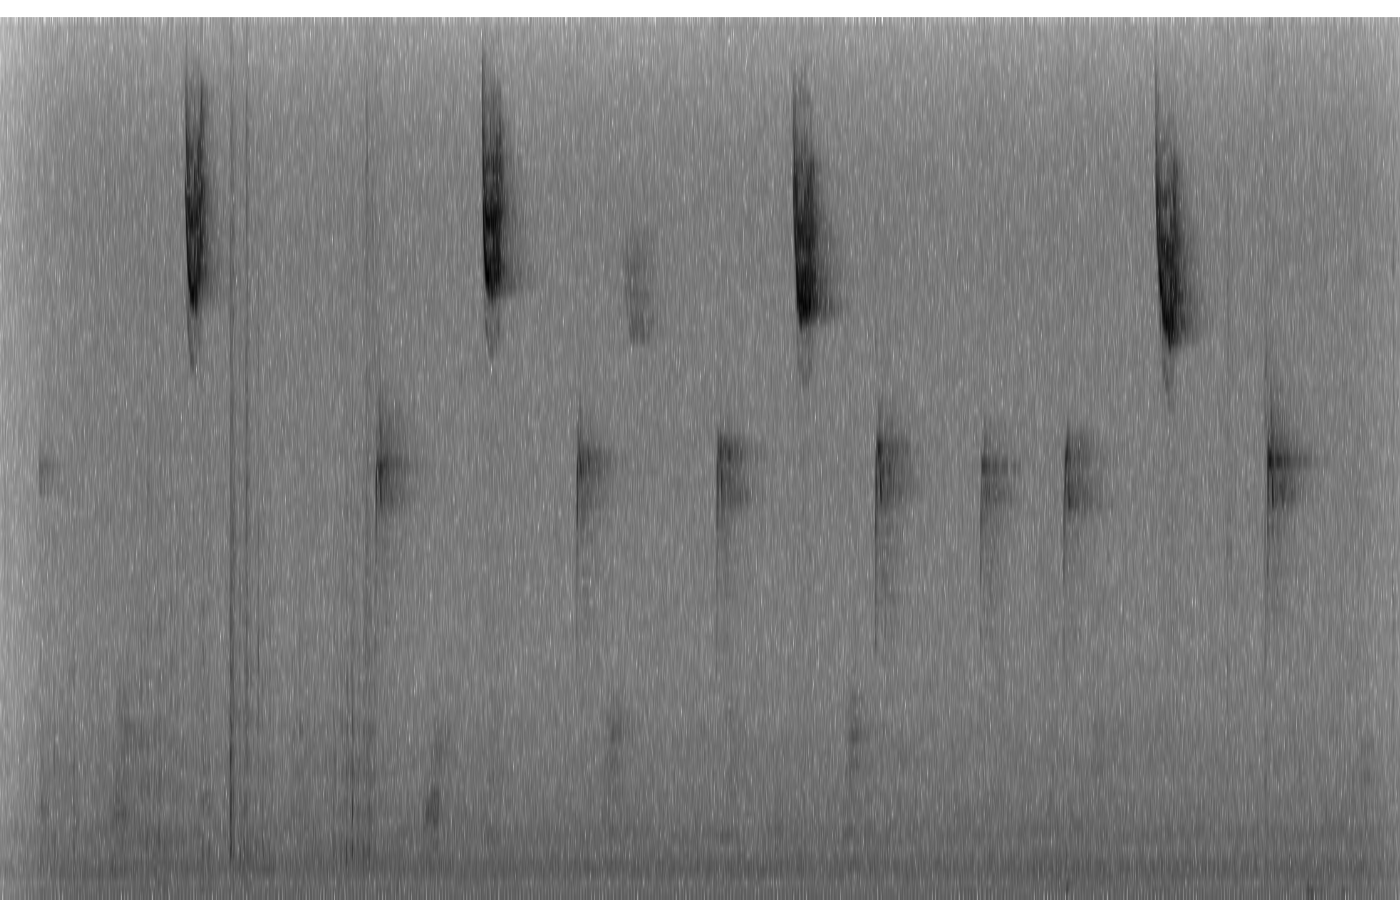
\includegraphics[height=1truein]{images/original}
\end{minipage}&
\begin{minipage}{1.8truein}
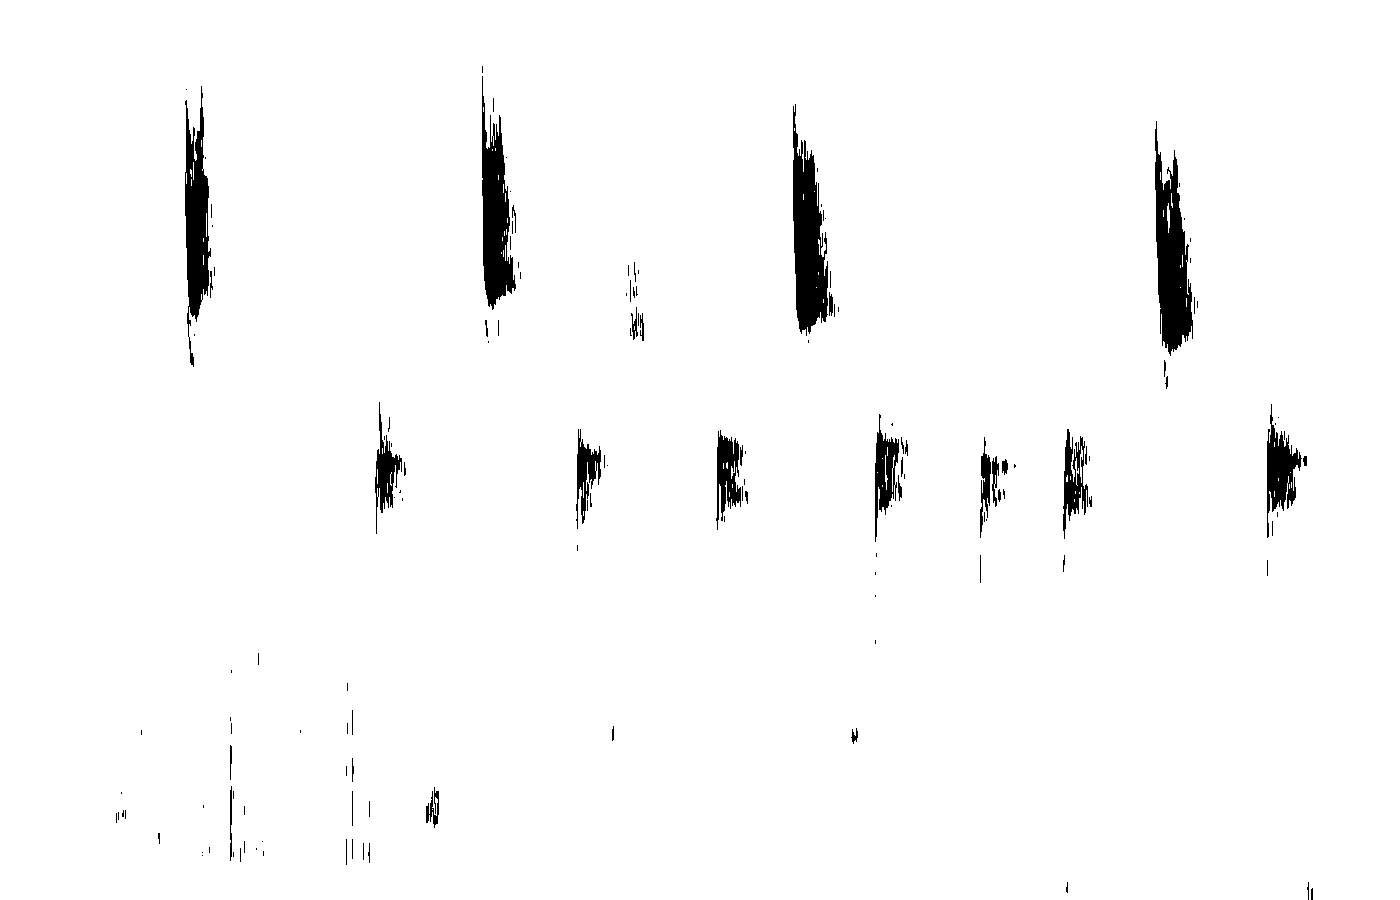
\includegraphics[height=1truein]{images/Median_clipped}
\end{minipage}\\
\smaller a. Original Spectrogram &\smaller b. Median Clipped\\
\begin{minipage}{1.8truein}
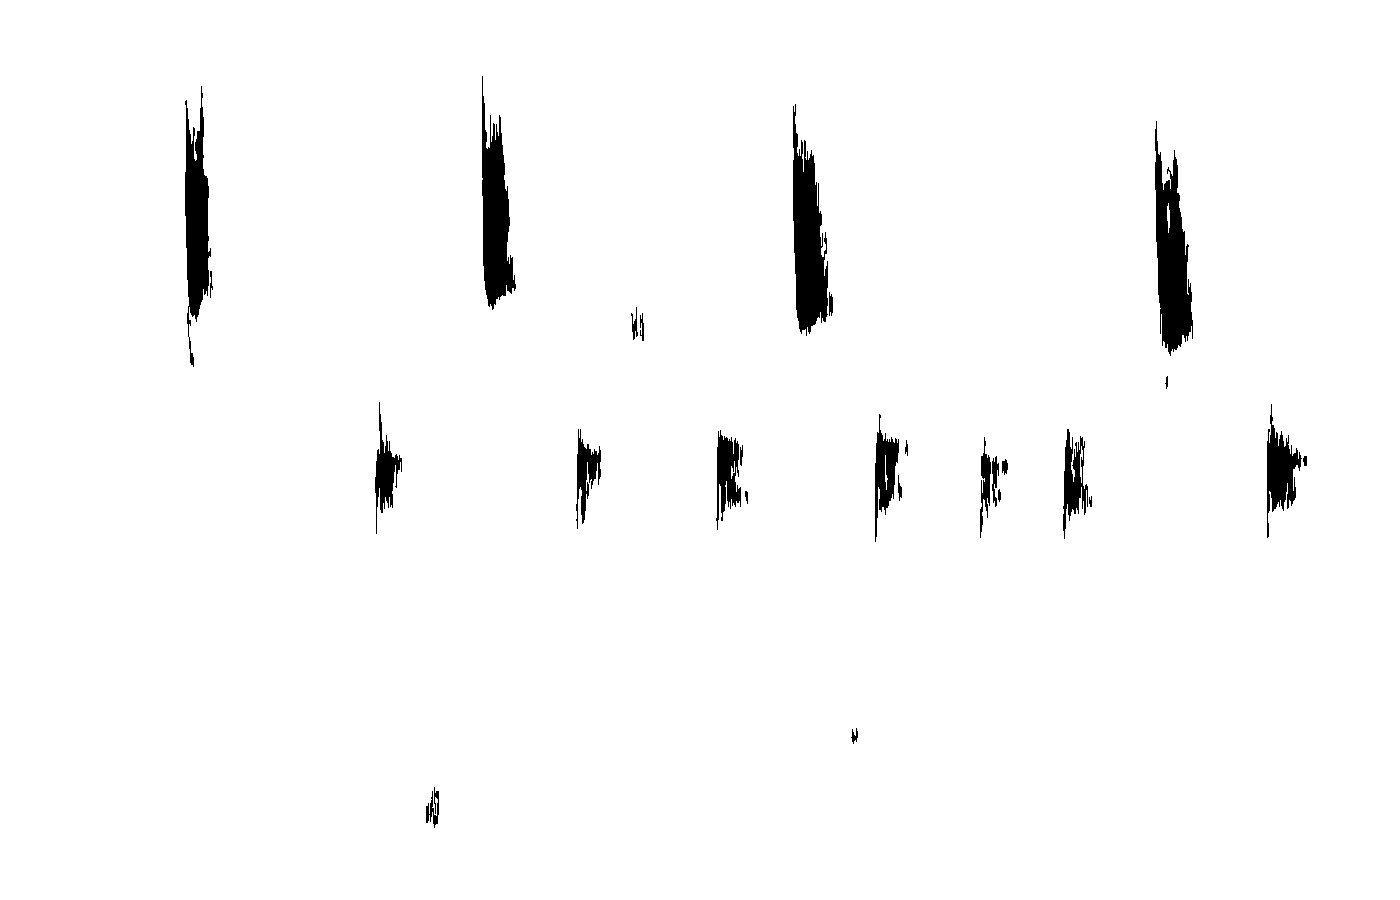
\includegraphics[height=1truein]{images/Eroded_and_propagated}
\end{minipage}&
\begin{minipage}{1.8truein}
\includegraphics[height=1truein]{images/labeled}
\end{minipage}\\
\smaller c.Eroded and Propagated &\smaller d. Labeled\\
\end{tabular}
\end{center}

}
%%%%%%%%%%%%%%%%%%%%%%%%%%%%%%%%%%%%%%%%%%%%%%%%%%%%%%%%%%%%%%%%%%%%%%%%%%%%%%
\headerbox{Classifiers/Ensembles}{name=Classifiers,column=1,below=Preprocessing}{
%%%%%%%%%%%%%%%%%%%%%%%%%%%%%%%%%%%%%%%%%%%%%%%%%%%%%%%%%%%%%%%%%%%%%%%%%%%%%%
The classifiers we used are

\textbf{Nearest Neighbor (NN).} We used euclidean and $\chi^2$ distance.

\textbf{Support Vector Machine (SVM).} This is the most common approach for multi-label classification. We tried linear SVM, sigmoid SVM and SVM with polynomial and rbf kernel.

%textbf{Support Vector Regression (SVR).} We use SVR to produce a soft output version of SVM

\textbf{Random Forest.} 
Random Forest is operated by constructing decision tree structure by the training examples. \
{\bf Ensemble Learning}=$<F\text{-strategy}(\tilde{K}), C\text{-strategy}, B\text{-strategy}, \bar{V}>$.


\begin{itemize}[noitemsep,topsep=1pt]
  \itemsep0.35em 
  \item $F\text{-strategy}$: return a binary array $F$ of chosen classifiers,  using nine measures of diversity, i.e., \emph{disagreement}, \emph{correlation}, \emph{Q-test}, \emph{double-fault}, \emph{coincident failure}, \emph{entropy}, \emph{interrater agreement}, \emph{Kohavi-Wolpert}, and \emph{generalized diversity}. 
  \item C\text{-strategy}: assign weights $C$, using \{\emph{uniform}, \emph{performance}, \emph{optimization}\}.
  \item B\text{-strategy}: obtain the belief matrix $B$, using \emph{basic} and \emph{new} forms.
  \item $\bar{V}$: enhance accuracy on more sure instances, leave others ``UNKNOWN''.
\end{itemize}


}
%%%%%%%%%%%%%%%%%%%%%%%%%%%%%%%%%%%%%%%%%%%%%%%%%%%%%%%%%%%%%%%%%%%%%%%%%%%%%%
\headerbox{Experiment}{name=references,column=0,span=2, below=Classifiers,below=Features, above=bottom}{
%%%%%%%%%%%%%%%%%%%%%%%%%%%%%%%%%%%%%%%%%%%%%%%%%%%%%%%%%%%%%%%%%%%%%%%%%%%%%%
\footnotesize
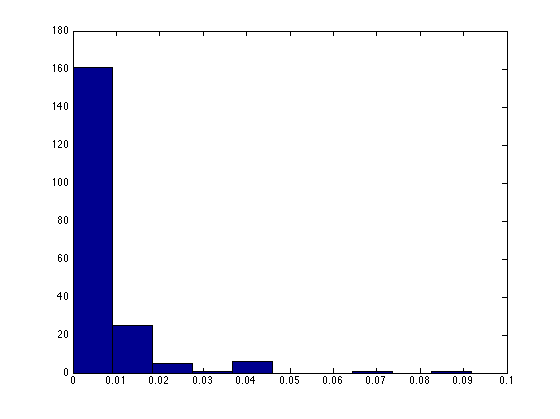
\includegraphics[width=0.3 \linewidth]{./images/Train_features.png}
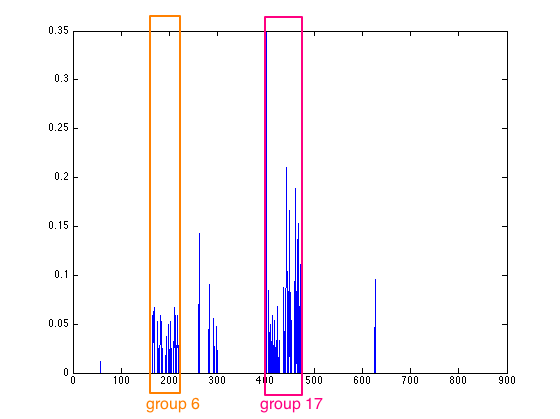
\includegraphics[width=0.3 \linewidth]{./images/mfcc_180.png}
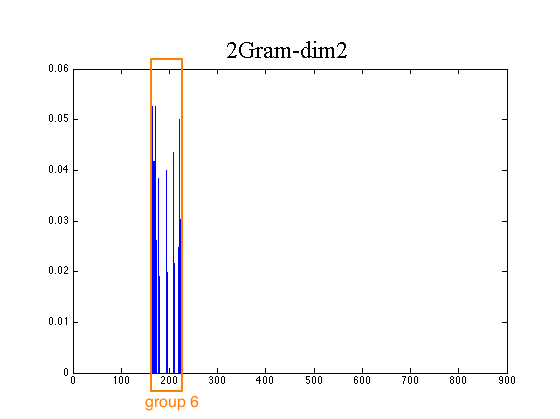
\includegraphics[width=0.32 \linewidth]{./images/ngram_202.png}\\
\footnotesize
Acuuracy of different classifier: \\
The accuarcy for classifier (using Random Forest) on mask descriptors by Briggs \emph{et al.} is 0.25. 


\begin{tabular}{cccc}
\multicolumn{1}{c}{\bf Classifier }&\multicolumn{1}{c}{\bf Accuracy}  &\multicolumn{1}{c}{\bf Features} &\multicolumn{1}{c}{\bf Settings}
\\ \hline \\
linear SVM		&67.7273/ 70.4545 		&BoW/ denoised 		&  \\
poly SVM		&69.0909/ 70.4545  	&BoW/ denoised  	& degree: 1  \\
			& 70 			& denoised BoW 	& degree: 2  \\
			& 70.4545  	& denoised BoW 	& degree: 3  \\
rbf SVM       	&70/ 	70.4545  	&BoW/ denoised 		&  \\
                     	&68  			&  BoW (log) 	&  \\
          		&76.8182  		&  denoised BoW 	&  $\gamma = 7.9433$ \\
          		&{\bf 78.1818}  	&  denoised BoW + 2gram 	&    \\
sigmoid SVM     	&70.9091/70.4545	&BoW/ denoised 		&  \\
random forest    	&57/63 			& BoW/ denoised 	& 100 trees; 5 splits \\
       			&63  			& denoised BoW 	& 100 trees; 2 splits \\
NN-euclidean   	&54.09/62.73		& BoW/ denoised 	&  \\
NN-chisquare	&62.27/71.82		& BoW/ denoised 	&  \\

\end{tabular}



\begin{center}
\begin{tabular}{cc}
\begin{minipage}{1.8truein}
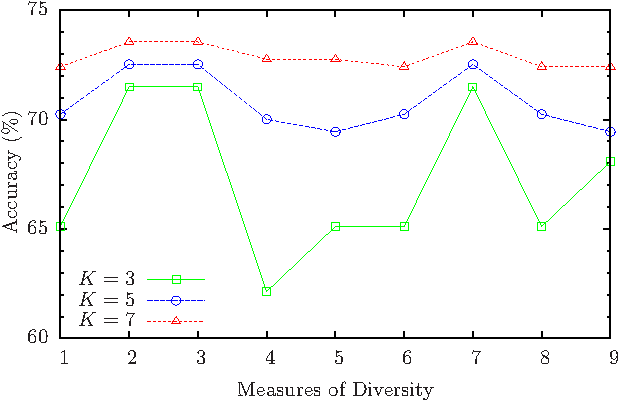
\includegraphics[height=1truein]{../Figure/diversity_k_train}
\end{minipage}&
\begin{minipage}{1.8truein}
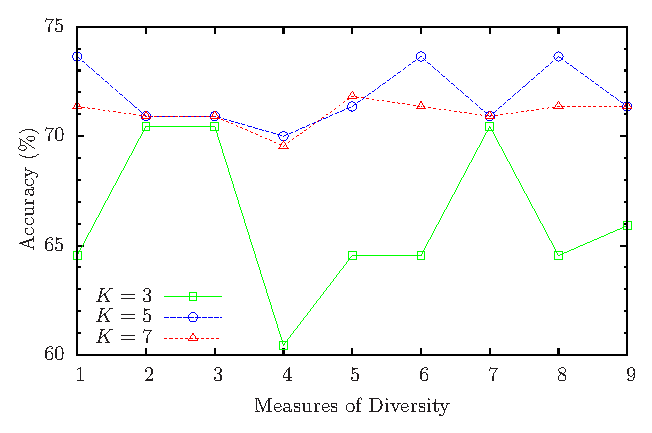
\includegraphics[height=1truein]{../Figure/diversity_k_test}
\end{minipage}\\
\smaller Training Accuracy &\smaller Testing Accuracy\\
\begin{minipage}{1.8truein}
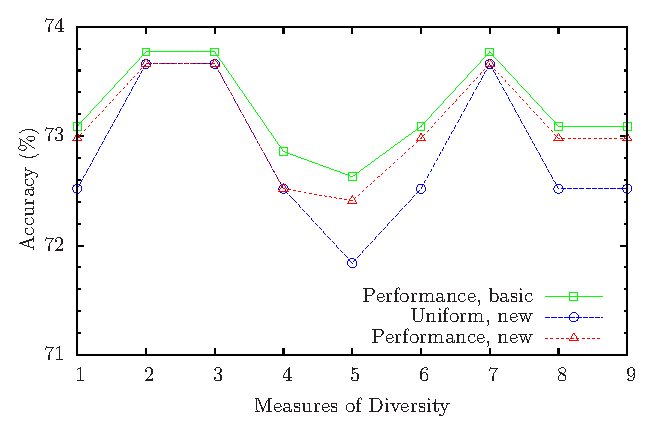
\includegraphics[height=1truein]{../Figure/diversity_7_others_train}
\end{minipage}&
\begin{minipage}{1.8truein}
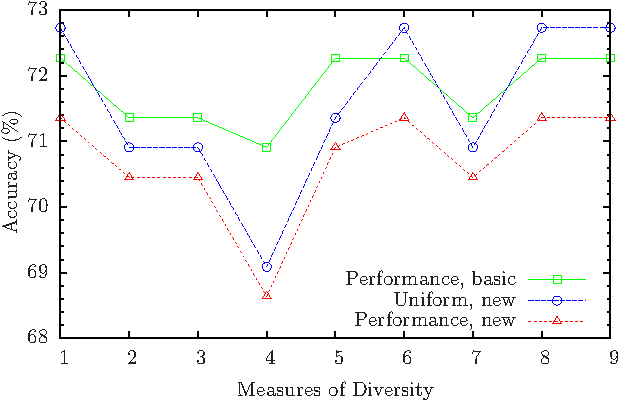
\includegraphics[height=1truein]{../Figure/diversity_7_others_test}
\end{minipage}\\
\smaller Training Accuracy &\smaller Testing Accuracy\\
\begin{minipage}{1.8truein}
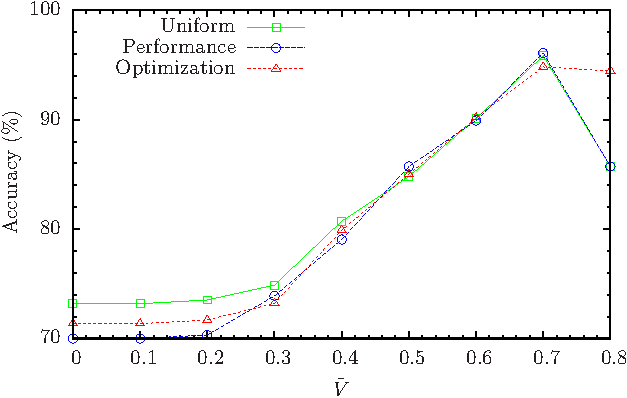
\includegraphics[height=1truein]{../Figure/threshould_accuracy}
\end{minipage}&
\begin{minipage}{1.8truein}
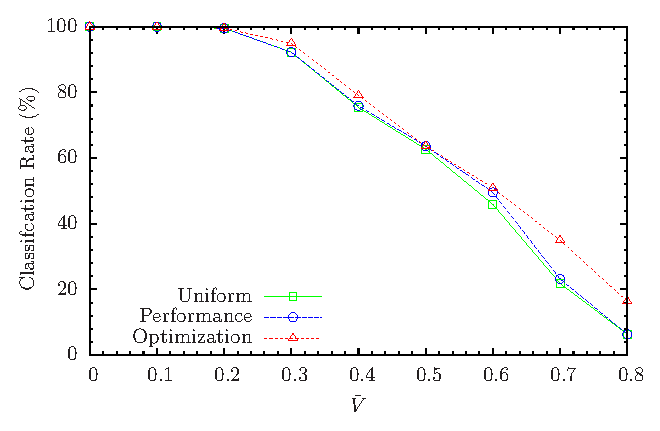
\includegraphics[height=1truein]{../Figure/threshould_rate}
\end{minipage}\\
\smaller Classification Accuracy &\smaller Classification Rate\\
\end{tabular}
\end{center}



}
%%%%%%%%%%%%%%%%%%%%%%%%%%%%%%%%%%%%%%%%%%%%%%%%%%%%%%%%%%%%%%%%%%%%%%%%%%%%%%

\end{poster}

\end{document}

